\subsection{Champs Magnétiques Intenses}
\begin{frame}{Laboratoire National des Champs Magn\'etiques Intenses}
  \begin{columns}[c]
    \begin{column}{0.5\textwidth}
      \begin{alertblock}{ \begin{small} Grand équipement francais (CNRS) \end{small}}
        \begin{small}
          \begin{itemize}
          \item Champs magnétiques intenses : à partir de 24 T.
          \end{itemize}
        \end{small}
      \end{alertblock}
    \end{column}
    \begin{column}{0.5\textwidth}
      \begin{alertblock}{}
        \begin{small}
          \begin{itemize}
          \item À Grenoble, champ continu max : 36 T
            (objectif 40-45T).
          \end{itemize}
        \end{small}
      \end{alertblock}
    \end{column}
  \end{columns}

  \vspace*{-0.4cm}
  \begin{tikzpicture}[scale=0.42][%
    >=latex,%
    font=\fontfamily{phv}\fontsize{7}{8}\selectfont,
    legend/.style={%
      draw,
      rounded corners=2pt,
      shade}]

    % frise 
    \draw[rounded corners,shade,left color=fColor!40,right color=fColor!5] (-14,0) -- ++ (26,0) -- ++ (1,1.5) -- ++(-1,1.5) -- ++ (-26,0) -- cycle;
    % axe bas
    \path (-10,0) -- (10,0) coordinate (xL axis);
    % axe haut
    \path[yshift=+3cm]         (-10,0) -- (10,0) coordinate (xH axis);
    % rupture
    \path[] (+0.5,-0.25) rectangle ++(8mm,3.5) node [midway,rotate=90,minimum width=3.5cm,shade,sharp corners,inner sep=1pt] (r1) {36 tesla};
    \draw[densely dotted] (r1.south east) -- (r1.south west) (r1.north east) -- (r1.north west);
    \draw[thick] (1.5,0) -- (1.5,-30mm) \bottomGraphics{width=3cm}{Figures/cmi/polyhelix.jpg};
    \draw[] (0,0) coordinate (an0) -- (an0 |- xH axis) -- ++ (0,2.5mm) node [above] {$10^0$};


    % scope 1
    \begin{scope}[xshift=3cm,xscale={14cm/400cm}]
      % graduation
      \draw[] (0,0)   coordinate (an0) -- (an0 |- xH axis) -- ++ (0,2.5mm) node [above] {$10^{+2}$};
      \draw[] (100,0) coordinate (an100) -- (an100 |- xH axis) -- ++ (0,2.5mm) node [above] {$10^{+3}$};
      \draw[] (200,0) coordinate (an200) -- (an200 |- xH axis) -- ++ (0,2.5mm) node [above] {$10^{+9}$};

      % evennement
      \topEvent{0,0}{an1617}{0,28mm} \topLegend{text width=4.5cm,name=r}{100 t :\\Pulsed magnetic field (ND) (USA)};
      \bottomEvent{127,0}{an1727}{0,-10mm} \bottomLegend{text width=4.5cm}{2800 t :\\Pulsed magnetic field (D) (Russia)};
      \topEvent{200,0}{an1617}{0,12mm} \topLegend{text width=2cm}{100 Mt to 100 Gt :\\Magnetar};
    \end{scope}

    % scope 2
    \begin{scope}[xshift=0cm,xscale={0.7cm/30cm}]
      % graduation
      \draw[] (-100,0) coordinate (anM1000) -- (anM1000 |- xH axis) -- ++ (0,2.5mm) node [above,fill=white] {$10^{-1}$};
      \draw[] (-200,0) coordinate (anM2000) -- (anM2000 |- xH axis) -- ++ (0,2.5mm) node [above,fill=white] {$10^{-2}$};
      \draw[] (-300,0) coordinate (anM3000) -- (anM3000 |- xH axis) -- ++ (0,2.5mm) node [above,fill=white] {$10^{-5}$};
      \draw[] (-500,0) coordinate (anM4000) -- (anM4000 |- xH axis) -- ++ (0,2.5mm) node [above,fill=white] {$10^{-12}$};
      % evennement

      \bottomEvent{6,0}{anM30}{0,-30mm} \bottomLegend{text width=2.5cm}{$1.5$ to 3 t : \\medical MRI systems};

      \topEvent{-173,0}{anM1730}{0,12mm} \topLegend{text width=2.5cm}{0.5 mt :\\limit for pacemakers};
      \bottomEvent{-300,0}{anM1730}{0,-10mm} \bottomLegend{text width=3cm}{31 to 100 $\mu$t :\\Earth's magnetic field};
      \topEvent{-500,0}{anM3730}{0,12mm} \topLegend{text width=2cm}{$10^{-12}$ t :\\Human brain};
    \end{scope}
  \end{tikzpicture}
\end{frame}

\begin{frame}{Laboratoire National des Champs Magn\'etiques Intenses}

   Installation champs pulsés à TOULOUSE : 14 MJ, 24 kV, 1 GW, 80 Tesla
   \vskip-0.3cm
   \begin{figure}[H]
    \centering
    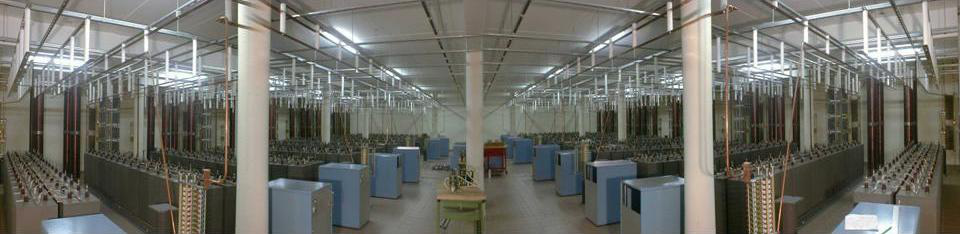
\includegraphics[scale=0.3]{Figures/cmi/powersupply_pulsed.png}
   \end{figure}

   Installation champs continus à GRENOBLE: 24 MW,  36 Tesla
   \vskip-0.3cm

 \begin{columns}[c]
  \begin{column}{8cm}
   \begin{figure}[H]
    \centering
    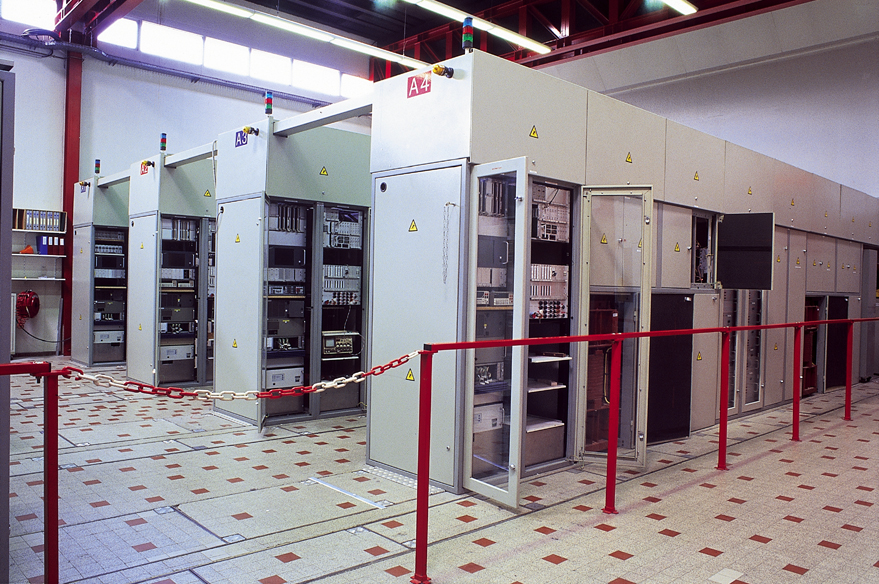
\includegraphics[scale=0.2]{Figures/cmi/powersupply.png}
   \end{figure}
  \end{column}

  \begin{column}{5cm}
   \begin{figure}[H]
    \centering
    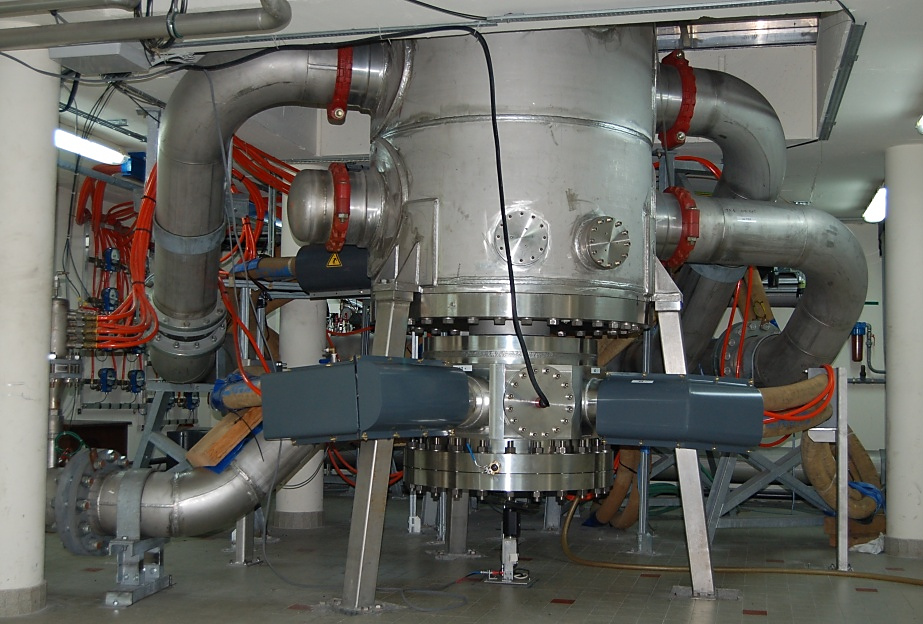
\includegraphics[scale=0.4]{Figures/cmi/magnet.png}
   \end{figure}
  \end{column}
 \end{columns}
\end{frame}

% \begin{frame}{Champs magnétiques intenses : domaines d'application}
%   \begin{columns}
%     \begin{column}{0.55\textwidth}
%       \begin{small}
%         \begin{itemize}
%         \item Supraconductivité appliquée ;
%         \item Science du magnétisme ;
%         \item (Bio-)Chimie ;
%         \end{itemize}
%       \end{small}

%     \end{column}

%     \begin{column}{0.55\textwidth}
%       \begin{small}
%         \begin{itemize}
%         \item Physique du solide (Résonance Magnétique Nucléaire) ;
%         \item Lévitation magnétique ;
%         \item ...
%         \end{itemize}
%       \end{small}

%     \end{column}
%   \end{columns}

%   \begin{figure}[H]
%     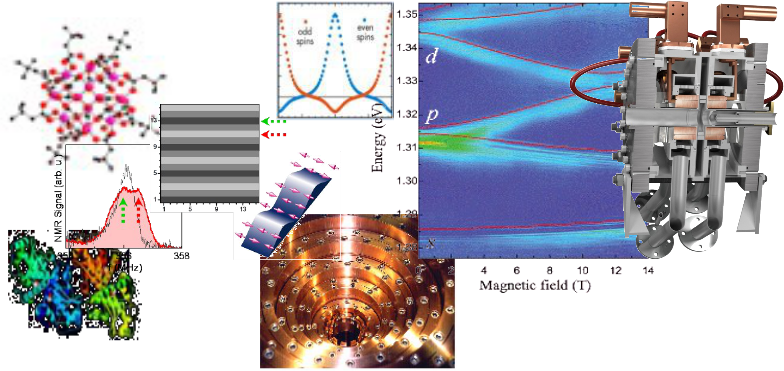
\includegraphics[scale=0.5]{Figures/cmi/research.png}
%   \end{figure}
% \end{frame}

\begin{frame}{Champs Magnétiques Intenses : à quoi ça sert ?}
    \begin{columns}[c]
      \begin{column}{0.78\textwidth}
        \begin{block}{Reproduire les conditions de zero-gravité}
          Moteur d'ariane 6 (SNECMA) : 
          \begin{itemize}
          \item Comment se comporte l'hydrogène liquide (carburant) en apesanteur ?
            \begin{itemize}
            \item Données d'entrée pour le design du moteur
            \item Moins coûteux qu'une expérience en conditions "réelles"
              \begin{itemize}
              \item heure de champ intense ($\approx$ 1000 \euro)
              \item vol parabolique ($\approx$ 100.000 \euro)
              \item vol dans l'espace ($\approx$ 10.000.000 \euro)
              \end{itemize}
            \end{itemize}
          \end{itemize}
          \vspace*{-0.4cm}
          \begin{columns}[c]
            \begin{column}{0.5\textwidth}
              \begin{figure}[H]
                \centering
                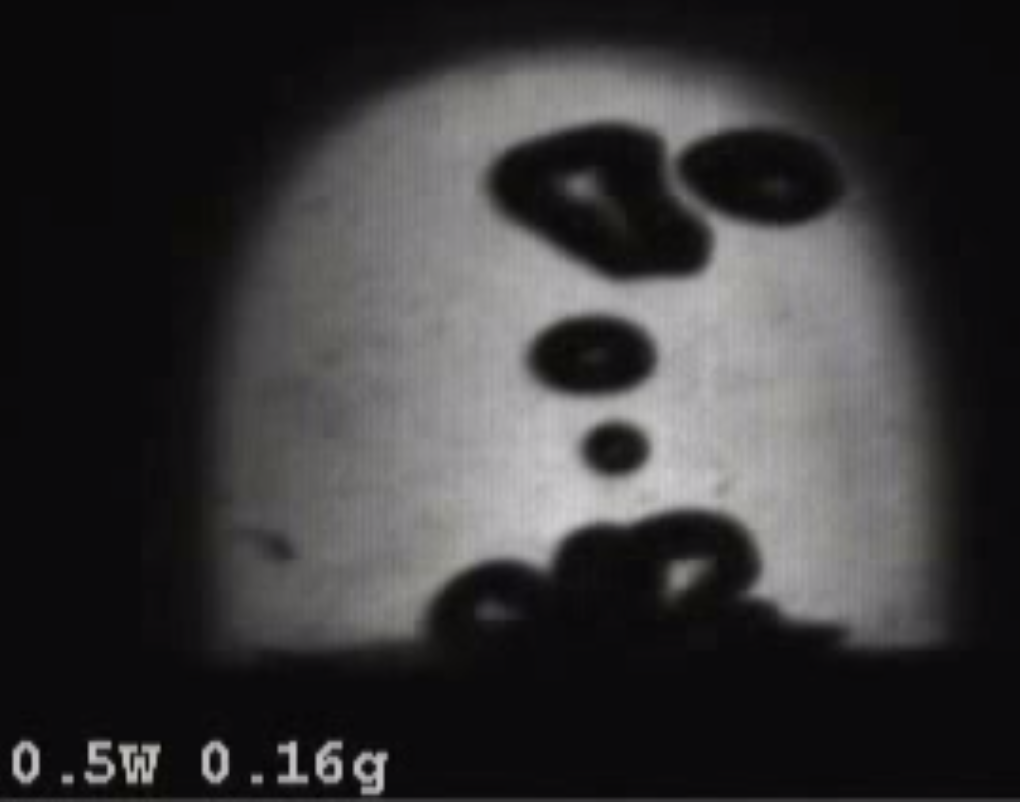
\includegraphics[scale=0.1]{Figures/cmi/levitation_1.png}
              \end{figure}
            \end{column}
            \begin{column}{0.5\textwidth}
              \begin{figure}[H]
                \centering
                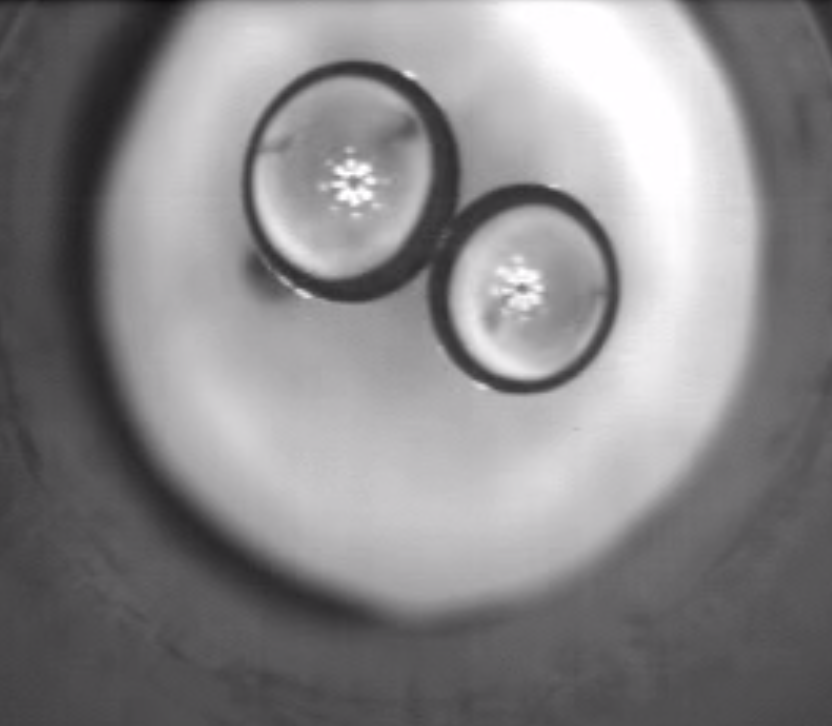
\includegraphics[scale=0.12]{Figures/cmi/levitation_2.png}
              \end{figure}
            \end{column}
          \end{columns}
        \end{block}
      \end{column}
      \begin{column}{0.25\textwidth}
        \begin{figure}[H]
          \centering
          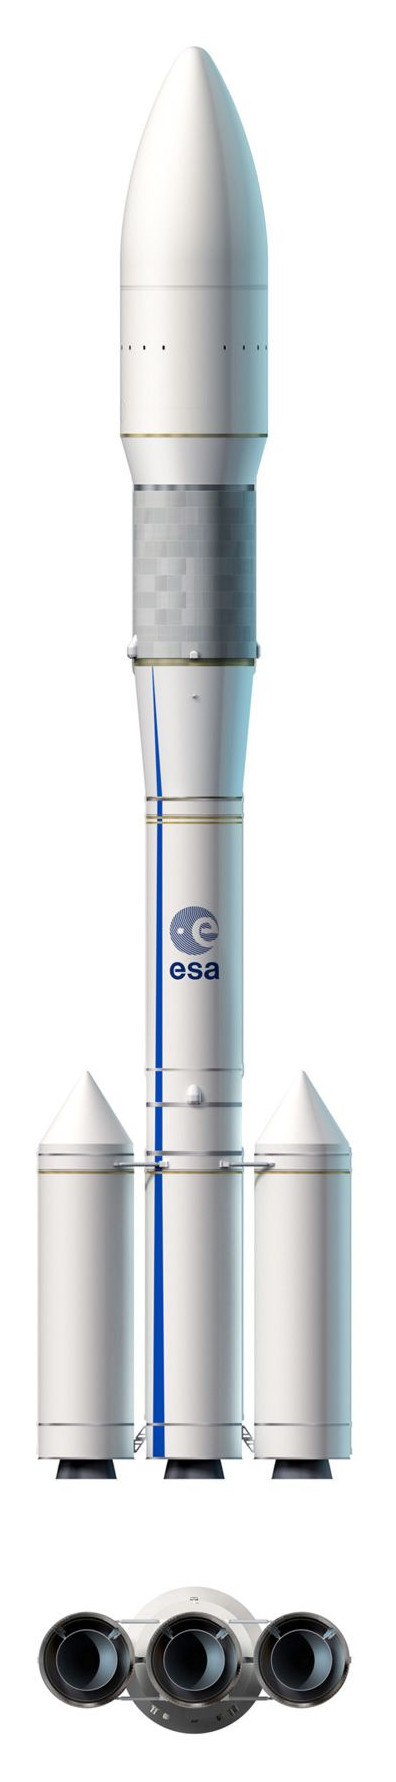
\includegraphics[scale=0.12]{Figures/cmi/ariane6_2.jpg}
        \end{figure}
      \end{column}
    \end{columns}
\end{frame}

\begin{frame}{Champs Magnétiques Intenses : à quoi ça sert ?}

  \begin{block}{Etudier les propriétés magnétiques}
    Optimisation de la capacité des disques durs
    \begin{itemize}
    \item Capacité dépend des propriétés magnétiques
      \begin{itemize}
      \item Revetement des disques : oxyde de fer (magnétique)
      \item Ecriture d'un bit : envoi d'une charge magnétique
      \item Lecture d'un bit : mesure de son champ magnétique
      \end{itemize}
    \end{itemize}
    \vspace*{-0.3cm}
    \begin{figure}[H]
      \centering
      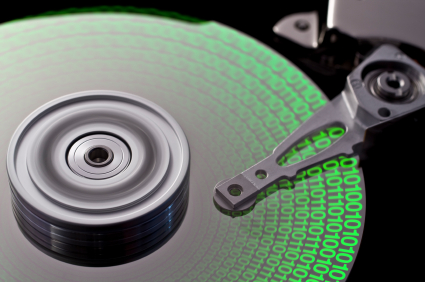
\includegraphics[scale=0.2]{Figures/cmi/disk.png}
    \end{figure}

    Compréhension/Optimisation des propriétés magnétiques :
    \vspace*{-0.2cm}
    \begin{center}
      Mega-octets (Mo) $~\longrightarrow~$ Giga-octets (Go) $~\longrightarrow~$ Tera-octets (To)
    \end{center}
  \end{block}

\end{frame}

\begin{frame}{Electro-Aimants : à quoi servent les modèles ?}
  \begin{block}{Avant la mise en service : Développement des aimants}
    \begin{small}
      \begin{itemize}
      \item Augmenter l'intensité du champ magnétique
      \item Améliorer sa qualité (homogénéité)
      \end{itemize}
    \end{small}
    \vspace*{-0.5cm}
    \begin{center} \textbf{Optimisation $\Rightarrow$ Modélisation (fine) des electro-aimants} \end{center}
    \vspace*{-0.3cm}
    \begin{small}
      \begin{itemize}
      \item Permet de couvrir une large gamme de paramètres
        \begin{itemize}
        \item Envisager autant de cas que l'on veut pour trouver le design "optimal"
        \end{itemize}
      \item Possibilité de prévoir/anticiper les scénarios "catastrophes"
        \begin{itemize}
        \item Et éviter la casse (très couteuse!)
        \end{itemize}
      \end{itemize}
    \end{small}
  \end{block}
\end{frame}

\begin{frame}{Electro-Aimants : à quoi servent les modèles ?}
  \begin{block}{Après la mise en service : Lors d'un incident}
    \begin{small}
      \begin{itemize}
      \item Identifier/Comprendre la cause de l'incident
        \begin{itemize}
        \item Temperature trop elevée ? Problème mécanique ?
        \end{itemize}
      \end{itemize}
      \begin{figure}[H]
        \centering
        
\includegraphics[scale=0.15]{Figures/cmi/loupe.jpg}
      \end{figure}
    \end{small}
    \vspace*{-0.4cm}
    \begin{center} \textbf{Analyse $\Rightarrow$ Reproduire l'incident par la simulation} \end{center}
    \vspace*{-0.4cm}
    \begin{small}
      \begin{itemize}
      \item Trouver une solution pour éviter que l'incident se reproduise : optimisation avant (re-) mise en service
      \end{itemize}
    \end{small}
  \end{block}
\end{frame}

%\subsection{Magnet study requires multi-physics modeling}
\begin{frame}{Electro-Aimants : un problème multi-physique}
  \vspace*{-0.5cm}
  \begin{columns}[c]
    \begin{column}{.7\linewidth}

      \begin{block}{Simulation des électro-aimants}
        \begin{itemize}
        \item Champs magnétique intense
          \begin{itemize}
          \item Densité de courant $j=-\sigma \nabla V$
          \item Électrostatique/Magnétostatique
          \end{itemize}

        \item Éffet Joule
          \begin{itemize}
          \item Dissipation de l'énergie thermique
          \item $\rightarrow$ \textcolor{red}{Température} \\
          \end{itemize}

        \item Refroidissement des électro-aimants
          \begin{itemize}
          \item Échanges thermiques entre le conducteur et l'eau
          \item $\rightarrow$ \textcolor{red}{Thermo-hydraulique } \\
          \end{itemize}

        \item Stress mécanique
          \begin{itemize}
            % \item Laplace force (induced by magnetic field)
          \item Forces de Lorentz, Dilatation thermique
          \item $\rightarrow$ \textcolor{red}{Mécanique - Elasticité} \\
          \end{itemize}
        \end{itemize}
      \end{block}

    \end{column}
    \begin{column}{.42\linewidth}
      \vspace*{-0.5cm}
      \begin{figure}[H]
        \centering
        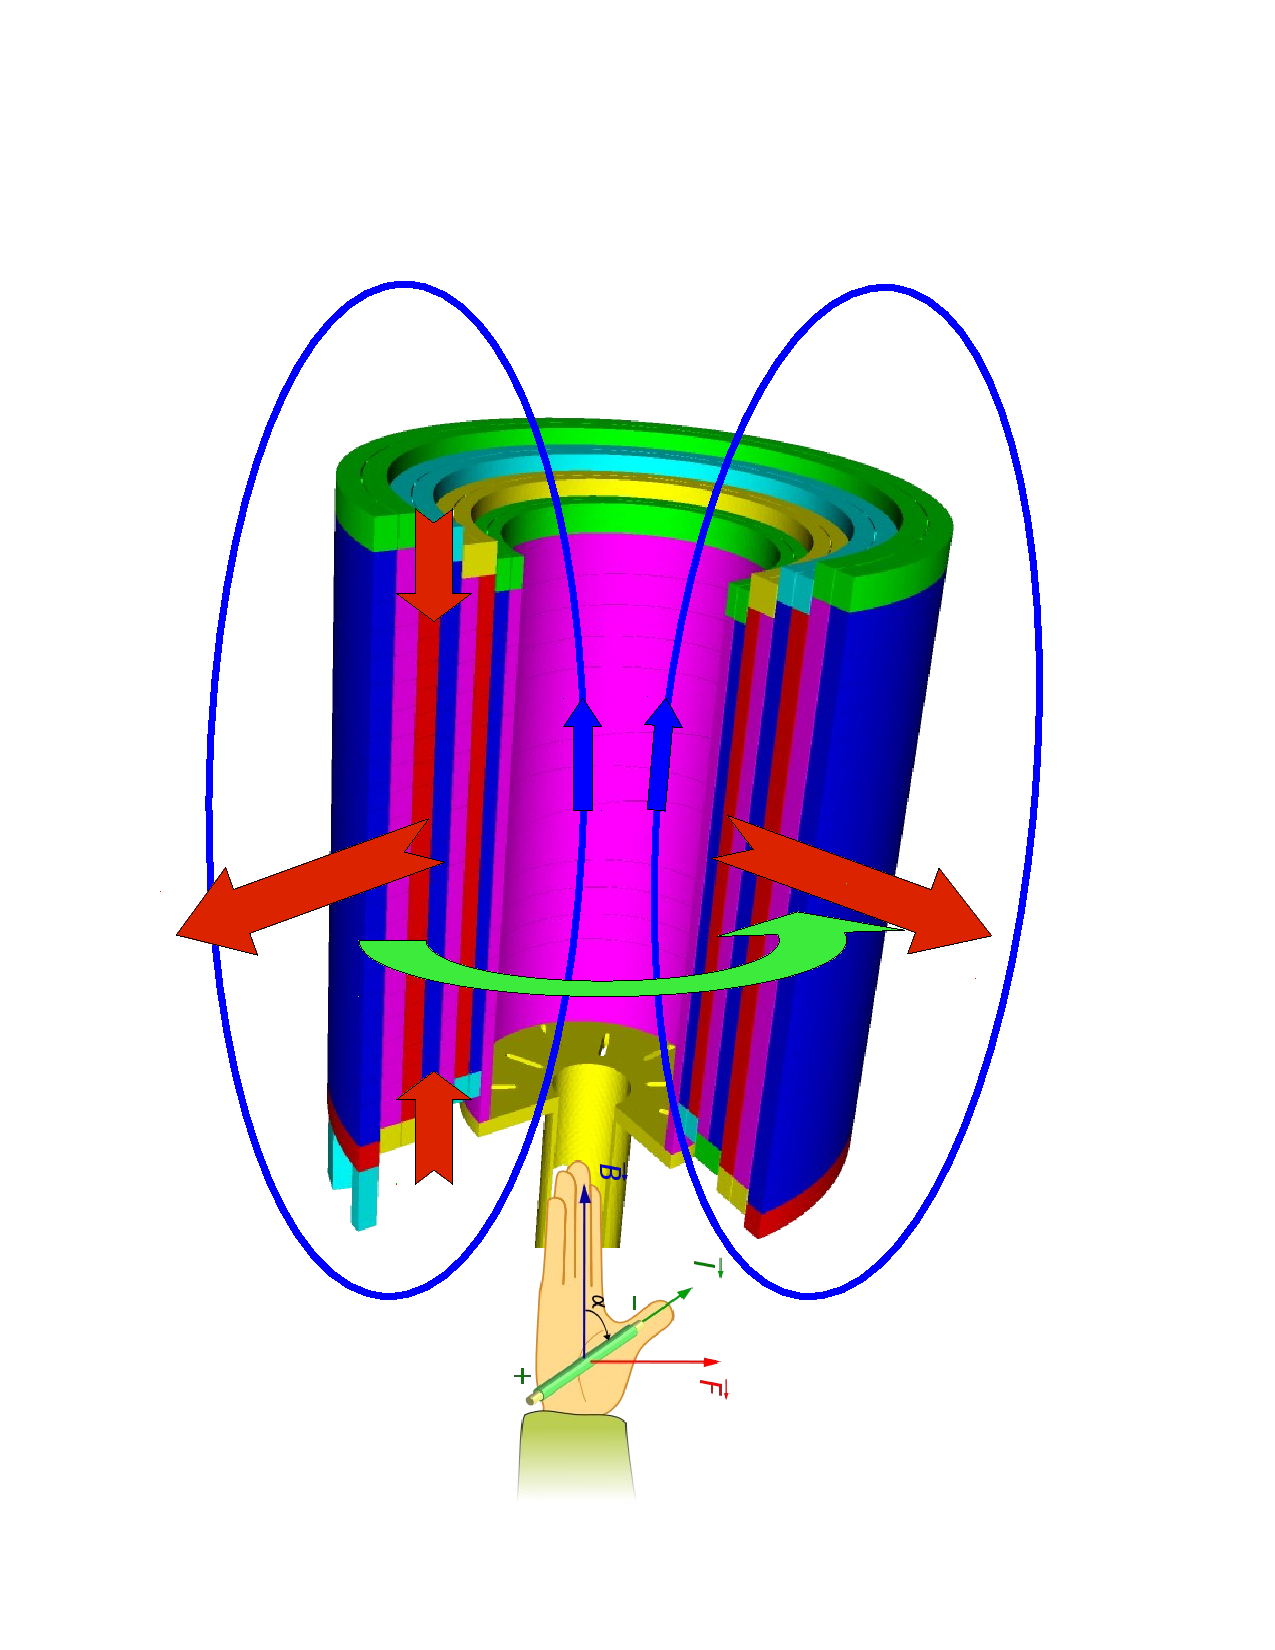
\includegraphics[scale=0.26]{Figures/cmi/Schema_Forces.pdf}
      \end{figure}
    \end{column}
  \end{columns}
\end{frame}

\begin{frame}{Electro-Aimants : objectifs pour le calcul}
  \begin{block}{Un modèle complet, précis, fiable et rapide}
    \vspace*{-0.3cm}
    \begin{columns}[c]
      \column{.47\linewidth}
      \begin{small}
        \begin{itemize}
        \item Hiérarchie de modèles
        \item Réduction de modèles (simulation temps réel fiable)
        \item Optimisation du design des électro-aimants
        \end{itemize}
      \end{small}
      \column{.49\linewidth}
      \begin{small}
        \begin{itemize}
        \item Contrôle  des électro-aimants
        \item Quantification d'incertitudes :
          \begin{itemize}
          \item Analyse de sensibilité
          \item Estimation de quantile
          \end{itemize}
        \item Optimisation sous incertitudes
        \end{itemize}
      \end{small}
    \end{columns}
  \end{block}
  
  \begin{columns}[c]
    \column{.1\linewidth}
    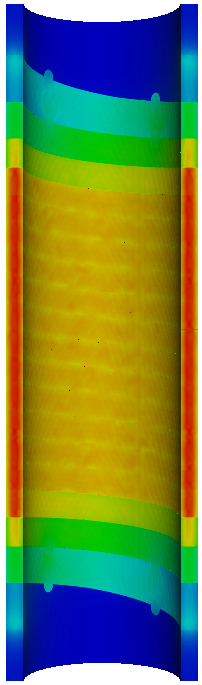
\includegraphics[height=.4\textheight]{Figures/cmi/temperature_newton_HL31_bmap+dilat_ws2.png}
    \column{.3\linewidth}
    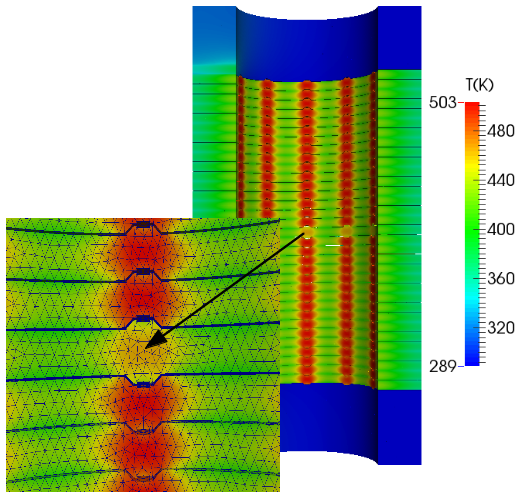
\includegraphics[height=.4\textheight]{Figures/cmi/temp_picard_np1024_OT200l170_comp.png}
    \column{.3\linewidth}
    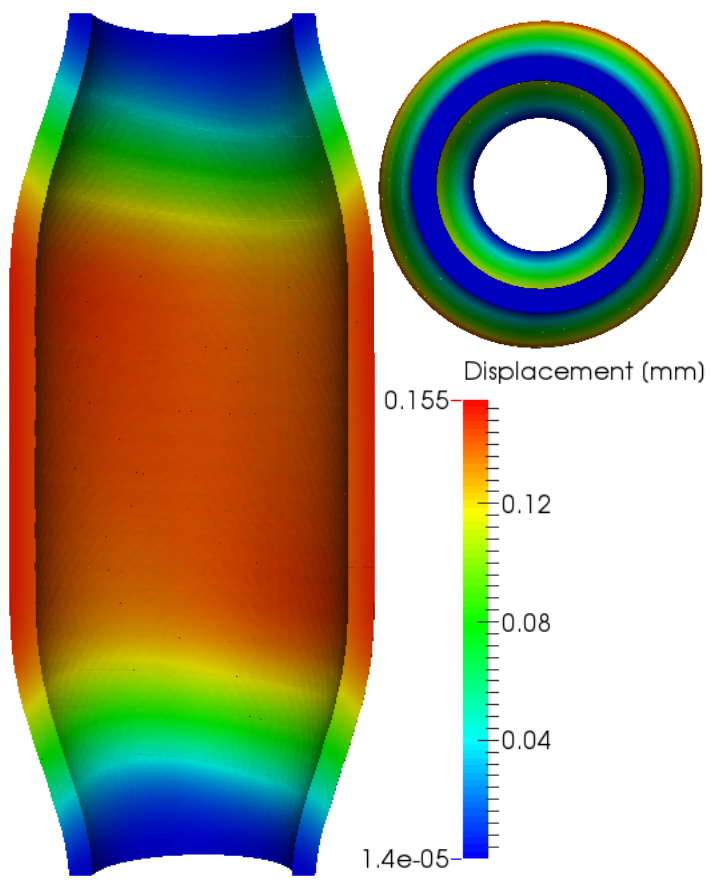
\includegraphics[height=.4\textheight]{Figures/cmi/Magnetmodels_bmap+dilat_HL31.png}
    \column{.19\linewidth}
    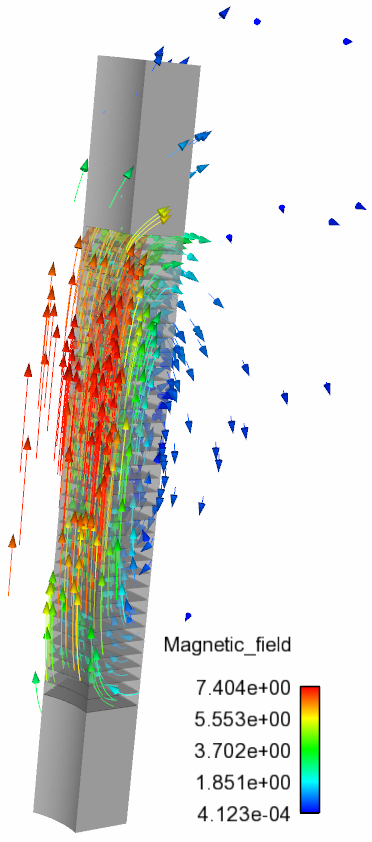
\includegraphics[height=.4\textheight]{Figures/cmi/HR-21-sector_magnetic_field_02.png}
  \end{columns}

\end{frame}

%%% Local Variables: 
%%% mode: latex
%%% TeX-master: "slides-math-formations-metiers"
%%% End: 
